\documentclass[xcolor=table]{beamer}

\usepackage{graphbox}       % For centre alignment of graphics
\usepackage{textcomp}       % Text companion fonts
\usepackage{tikz}

\setbeamertemplate{navigation symbols}{}
% \setbeamertemplate{items}[circle]

\hyphenpenalty 4000 \sloppy


\title{Bunch-by-Bunch Processing \\on MicroTCA at Diamond}
\author{Michael Abbott}
\institute{Diamond Light Source}
\date{Thursday 19\textsuperscript{th} April 2018}


\newcommand{\cc}{\cellcolor{green!60!blue!20}}

\begin{document}

\frame{\titlepage}


% ------------------------------------------------------------------------------
%
\begin{frame}{Scope of this talk}

I will talk about signal processing for Multi-Bunch Feedback

\begin{itemize}
\item Focus on digital chain of bunch-by-bunch processing
\item Input and output at up to 500\,MHz, baseband, taken as given
\item Assume pickups, front-ends, amplifiers, transducers, etc already given
\end{itemize}

Focus will be on applications and capabilities.

\end{frame}


% ------------------------------------------------------------------------------
%
\begin{frame}{Applications}
Applications of MBF (Multi-Bunch Feedback) system

\begin{itemize}
\item Beam stabilisation
\item Tune measurement
\item Diagnostics and Machine Physics experiments
\item Post-Mortem Analysis
\end{itemize}

\end{frame}


% ------------------------------------------------------------------------------
%
\begin{frame}{History of MBF at DLS}

\footnotesize

The immediate precursor to Multi-Bunch Feedback at Diamond Light Source is:

\begin{itemize}
\item ESRF, Eric Plouviez et al., reported 2006, implemented on the Libera
    platform, written using Xilinx System Generator.
\end{itemize}

At Diamond the following evolution occurred:

\begin{itemize}
\item Converted from System Generator to System Verilog by Isa Uzun, and tune
    sweep and individual bunch control added, reported 2008.
\item Substantial rework by myself and Isa, reported 2013, introduction of
    sequencer and bunch bank control.
\item Converted to VHDL to avoid licensing problems, adopted by ALBA 2014.
\item Rewritten and ported to MicroTCA COTS hardware, 2016 to present.
\end{itemize}

\end{frame}


% ------------------------------------------------------------------------------
%
\begin{frame}{MBF on MicroTCA}

The Libera platform is based on 15 year old hardware, and our FPGA is full.
Using MicroTCA lets us use modern Commercial Off The Shelf hardware for data
acquisition, signal processing, control.

\begin{description}
\item[FPGA carrier]
    Vadatech AMC525 provides a Virtex-690 FPGA (with 3,600 DSP units), 2GB of
    fast RAM, 8 lane PCIe3 interconnect, support for 2 FMC cards
\item[ADC/DAC FMC]
    Dual 14-bit 500 M\,Hz ADC and 16-bit DAC.
\end{description}

This platform gives us plenty of room and allows for high performance, in
particular the 8$\times$PCIe3 readout of captured memory is valuable.

\end{frame}


% ------------------------------------------------------------------------------
%
\begin{frame}{Capabilities of DLS MBF}

\begin{itemize}
\item Bunch by bunch feedback with 16-tap FIR per bunch
\item Up to four different FIRs selectable for different bunches
\item ADC compensation and DAC pre-emphasis with FIR
\item Dynamic view of bunch motion: min, max, mean, variance
\item Programmable sequencer with swept NCO excitation and synchronous detector
\item Capture and fast readout of up to 1 second (2\,GB) of dual channel bunch
    by bunch data
\item Longitudinal feedback supported via bunch by bunch downsampling on FIR and
    90\textdegree{} channel phasing for IQ output
\end{itemize}

\end{frame}


% ------------------------------------------------------------------------------
%
\begin{frame}{Signal Processing Chain}

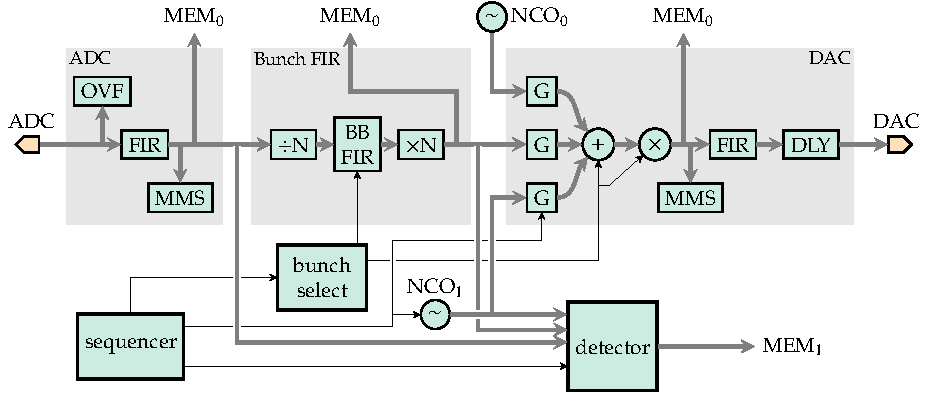
\includegraphics[width=\linewidth]{processing.pdf}

\end{frame}


% ------------------------------------------------------------------------------
%
\begin{frame}{Min/Max/Sum (MMS)}

\tikz[remember picture, overlay]
\node[anchor=north east] at (current page.north east) {
    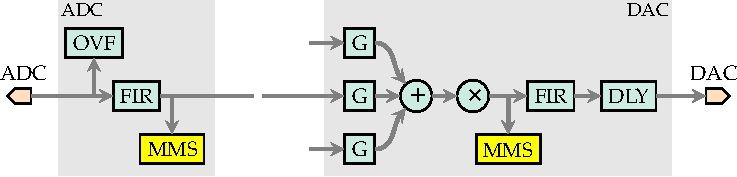
\includegraphics[width=5.5cm]{mms-ctxt.pdf}};

The MMS unit accumulates statistics for every bunch, which are then read out
periodically (the default interval is 200\,ms) and used to display the following
overview information:

\begin{itemize}
\item Overall extent of beam motion (max${}-{}$min)
\item Standard deviation of beam motion
\item Average beam position
\end{itemize}

\makebox[\linewidth]{
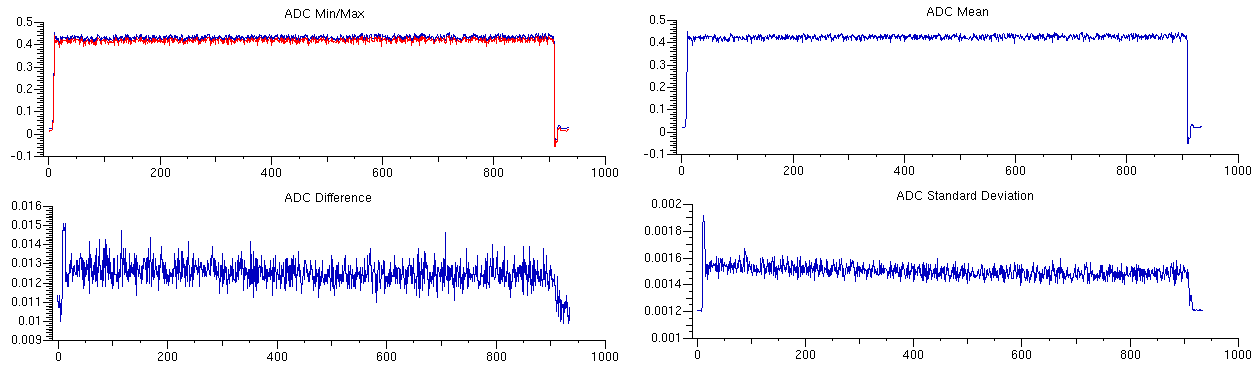
\includegraphics[width=\paperwidth]{mms2.png}
}

\footnotesize
Sample size: 100,000 turns, note standard deviation $\approx$ 10\,\%
peak-to-peak

\end{frame}


% ------------------------------------------------------------------------------
%
\begin{frame}{Sequencer and Bunch Select}

\tikz[remember picture, overlay]
\node[anchor=north east] at (current page.north east) {
    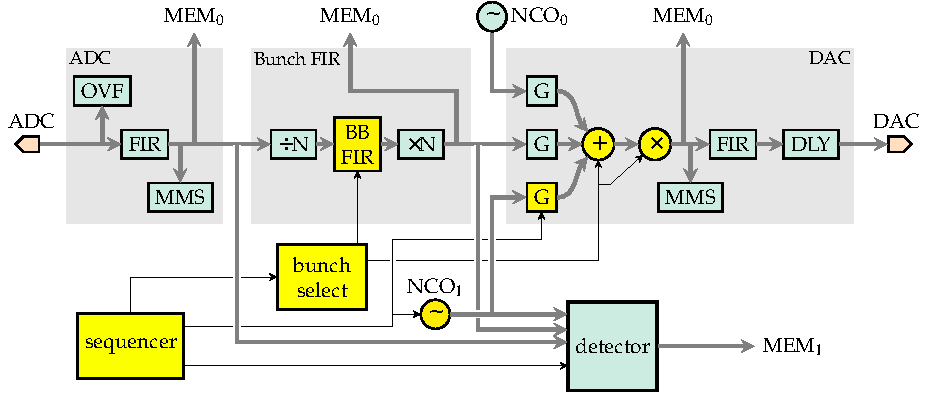
\includegraphics[width=5.5cm]{seq-ctxt.pdf}};

The Bunch Select unit selects for each bunch:
\begin{itemize}
\item Which of 4 FIRs to use on that bunch
\item What combination of outputs for that bunch (NCOs and FIR)
\item Overall bunch gain
\end{itemize}

The Sequencer provides up to 7 states to control:
\begin{itemize}
\item Sweep control (NCO frequency range, sweep rate, etc)
\item Which of 4 bunch configurations to use
\end{itemize}

The Super Sequencer repeats a sequencer experiment for up to 1024 different
frequency offsets; this is particularly useful for mode scan experiments.

\end{frame}


% ------------------------------------------------------------------------------
%
\begin{frame}{Detector}

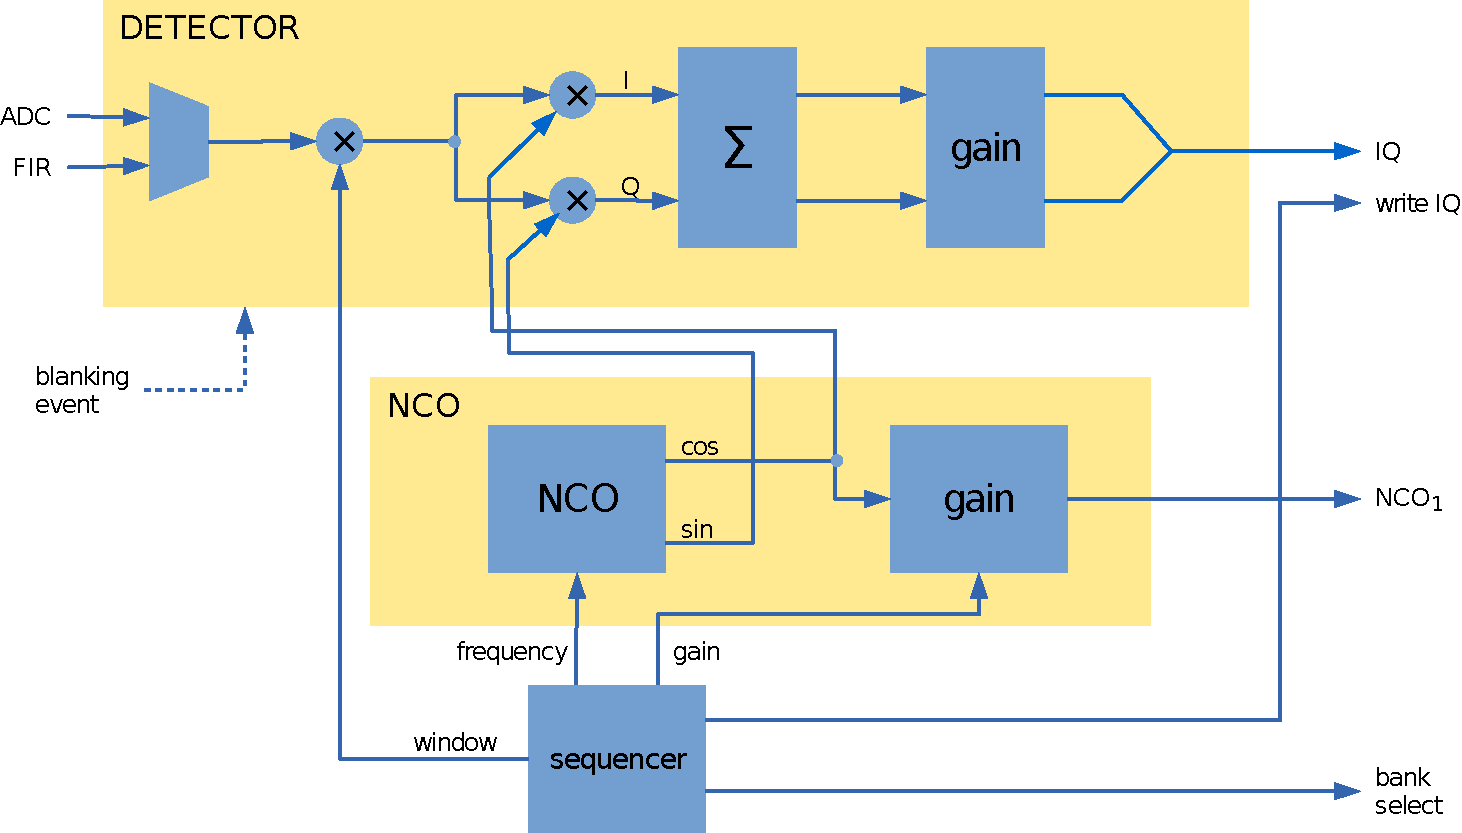
\includegraphics[width=\linewidth]{detector.pdf}

\end{frame}


% ------------------------------------------------------------------------------
%
\begin{frame}{Tune Sweep}

Examples of horizontal, vertical, and longitudinal tune sweeps with fitted
models.

\makebox[\linewidth]{
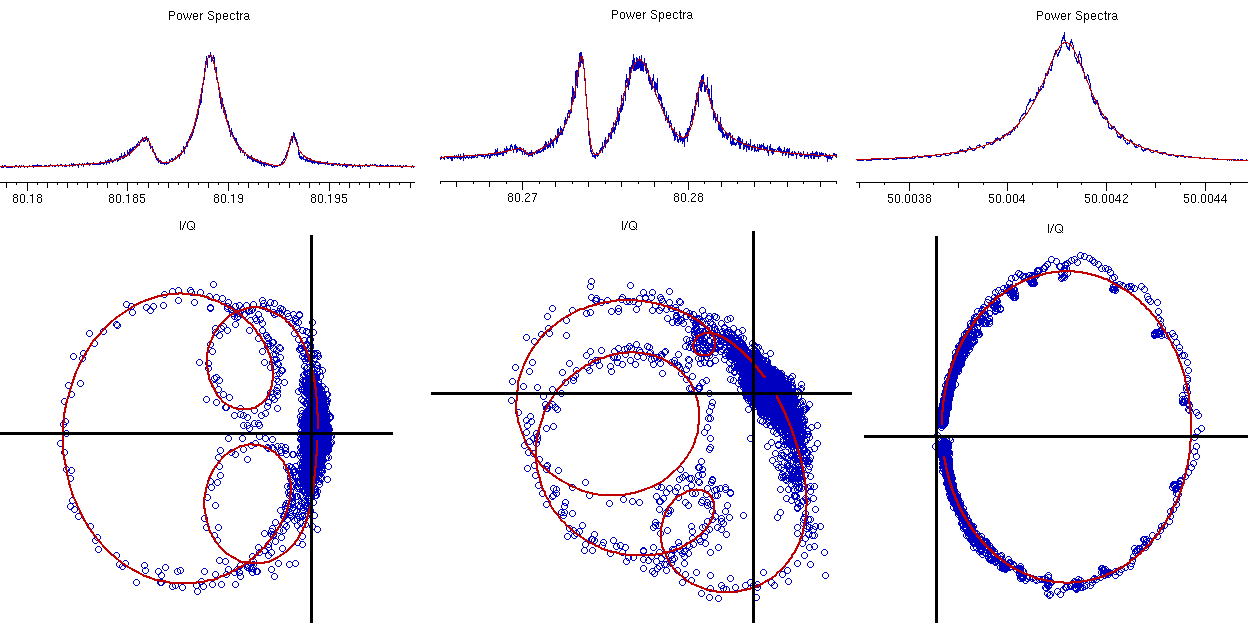
\includegraphics[width=\paperwidth]{tune.png}
}

\end{frame}


% ------------------------------------------------------------------------------
%
\begin{frame}{Longitudinal Mode Sweep Experiment}

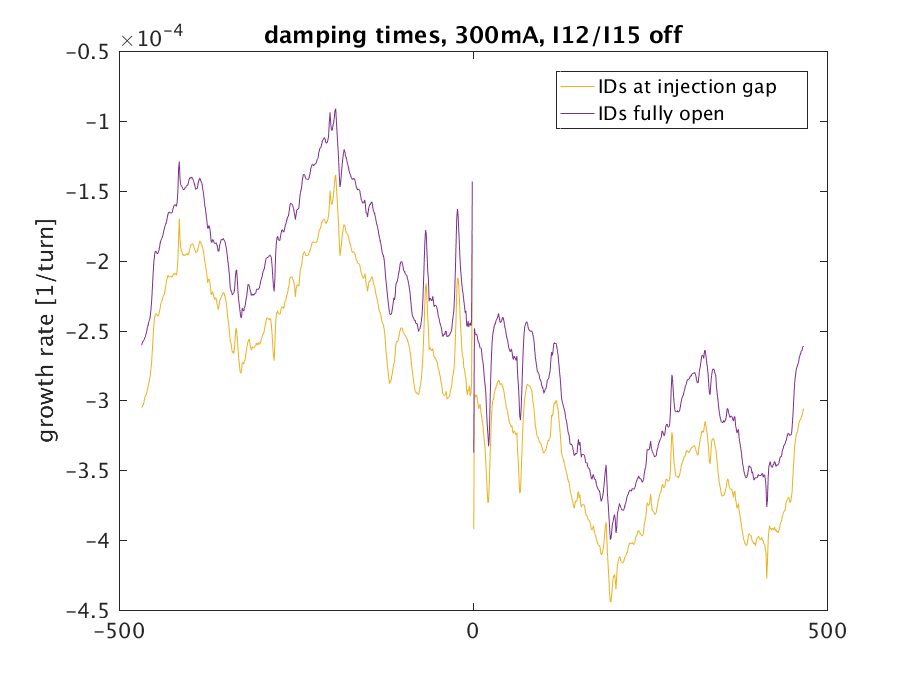
\includegraphics[width=\linewidth]{mode_sweep.png}

\end{frame}


% ------------------------------------------------------------------------------
%
\begin{frame}{Sequencer Setup for Sweep}

\begin{center}
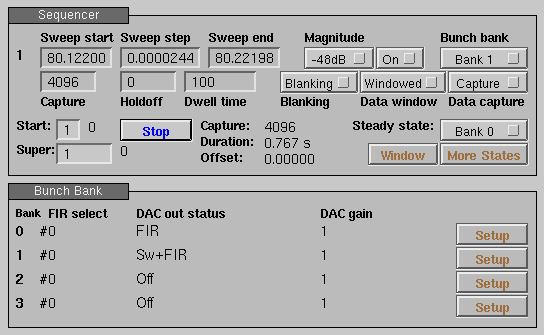
\includegraphics[width=0.8\linewidth]{control.png}
\end{center}

\end{frame}


% ------------------------------------------------------------------------------
%
\begin{frame}{Future Developments}

Three developments are planned for the immediate future

\begin{itemize}
\item Reimplement phase locked tune tracking on new system
\item Use PLL tune tracking to compensate for tune drifting during experiments
\item
    Provide functionality for playing precomputed data on to the beam.  Possible
    applications include:
    \begin{itemize}
    \item Feed forward correction of injection transients
    \item Narrow band noise excitation for tune sweep
    \end{itemize}
\end{itemize}

\end{frame}

\end{document}


% ------------------------------------------------------------------------------
%
\begin{frame}{}

\end{frame}
